\documentclass[12pt, a4paper, brazil]{article}

% --- PACOTES ---
\usepackage[utf8]{inputenc}
\usepackage[T1]{fontenc}
\usepackage[brazil]{babel}
\usepackage{graphicx}
\usepackage[a4paper, left=3cm, top=3cm, right=2cm, bottom=2cm]{geometry}
\usepackage{setspace}
\usepackage{indentfirst}
\usepackage{booktabs}
\usepackage{caption}
\usepackage[colorlinks=true, allcolors=black]{hyperref}
\usepackage{float}
\usepackage{hyperref}
\usepackage{listings}
\usepackage{xcolor} % Para definir cores de realce

% Configuração de cores e estilos para o código
\definecolor{fundo}{rgb}{0.96, 0.96, 0.96}
\definecolor{comentario}{rgb}{0.0, 0.5, 0.0}
\definecolor{palavra_chave}{rgb}{0.0, 0.0, 0.8}
\definecolor{texto_string}{rgb}{0.6, 0.1, 0.1}

\lstset{
    backgroundcolor=\color{fundo},
    basicstyle=\ttfamily\small, % Fonte monoespaçada para o código
    commentstyle=\color{comentario},
    keywordstyle=\color{palavra_chave}\bfseries,
    stringstyle=\color{texto_string},
    numbers=left,               % Números das linhas à esquerda
    numberstyle=\tiny\color{gray},
    stepnumber=1,
    frame=single,               % Moldura ao redor do bloco
    breaklines=true,            % Quebra linhas longas automaticamente
    showstringspaces=false
}

% Renomeia a legenda para o padrão em português (ABNT)
\renewcommand{\lstlistingname}{Código}
\renewcommand{\lstlistlistingname}{Lista de Códigos}

% --- CONFIGURAÇÕES DE TEXTO ---
\onehalfspacing 
\setlength{\parindent}{1.5cm} 

\begin{document}
\sloppy 

% --- 1. CAPA ---
\begin{titlepage}
    \begin{center}
        
\includegraphics[width=5cm]{estacio.png}
        \vspace{0.5cm}
    \end{center}
    \begin{center}
        \begin{minipage}{0.2\textwidth}
            % Sobe a imagem com o nome 'logo_ufpi.png'
            %
\includegraphics[width=2.5cm]{estacio.png} 
        \end{minipage}
        \begin{minipage}{0.7\textwidth}
            \centering
            {\small \textbf{CENTRO UNIVERSITÁRIO ESTÁCIO DE SÁ}} \\
            {\small \textbf{CAMPUS TERESINA}} \\
             {\small Data de entrega: 15 de junho de 2026} \\

        \end{minipage}
        
        \vspace{7cm}
        
        {\large \textbf{SISTEMA DE CADASTRO DE PRODUTOS}} \\
        {\small Disciplina: Programação de Software Básico em C} \\
        {\small Turma: 2026.1}
        
        \vspace{2cm}
        
        {\small 
\vspace{4cm}
        Gabriel de Oliveira Barbosa\\
        -\\
        -\\}      
        \vspace{1cm}
        {\small
        Prof. -}
      
        \vfill
        {\small \textbf{Teresina – PI}} \\
        {\small \textbf{15 de junho 2026}}
    \end{center}
\end{titlepage}

% --- 3. SUMÁRIO ---
\newpage
\tableofcontents
\newpage

% --- 4. DIAGNÓSTICO E TEORIZAÇÃO ---
\section{INTRODUÇÃO}

\subsection{Qual problema o programa procura resolver?}

O programa foi desenvolvido para resolver o problema do controle básico de estoque de produtos em uma empresa, loja ou estabelecimento comercial. Ele permite registrar informações importantes sobre cada produto, como código, nome, preço e quantidade disponível. Dessa forma, os dados ficam organizados e podem ser consultados posteriormente de maneira simples e rápida.

Além do cadastro, o sistema também auxilia no gerenciamento do estoque ao calcular automaticamente o valor total armazenado em produtos. Isso permite que o usuário tenha uma visão geral do capital investido no estoque. O programa ainda identifica qual produto possui o maior preço entre os cadastrados, fornecendo informações úteis para análises e tomadas de decisão relacionadas ao negócio.


\subsection{Qual é a finalidade do cadastro de produtos?}

A finalidade do cadastro de produtos é armazenar informações essenciais sobre os itens que compõem o estoque da empresa. Cada produto recebe um código de identificação, um nome, um preço e uma quantidade disponível, permitindo um controle mais eficiente dos recursos disponíveis para venda ou uso.

Com essas informações registradas, o usuário pode consultar os produtos cadastrados sempre que necessário. Isso facilita a organização do estoque, reduz a possibilidade de erros e melhora o acompanhamento dos produtos existentes. Além disso, o cadastro serve como base para os cálculos realizados pelo sistema, como o valor total do estoque e a identificação do produto mais caro.

\subsection{Quais conteúdos da linguagem C foram utilizados?}

O programa utiliza diversos conceitos fundamentais da linguagem C. Entre eles estão estruturas (\textit{struct}), funções, vetores, ponteiros, alocação dinâmica de memória, entrada e saída de dados com \textit{scanf} e \textit{printf}, além de bibliotecas como \textit{stdio.h}, \textit{stdlib.h} e \textit{string.h}.

Também são utilizados laços de repetição \textit{for}, estruturas condicionais \textit{if}, manipulação de strings com \textit{fgets} e \textit{strcspn}, além de operações matemáticas para calcular valores do estoque. Esses recursos tornam o programa mais organizado e eficiente.

% --- 5. PLANEJAMENTO E DESENVOLVIMENTO ---
\section{DESCRIÇÃO DO FUNCIONAMENTO}
\subsection{Como a quantidade de produtos é informada?}

A quantidade de produtos é informada pelo próprio usuário no início da execução do programa. O sistema solicita que seja digitado um valor entre 1 e 10, representando quantos produtos serão cadastrados.
Após a entrada do valor por meio do comando \textit{scanf}, o programa verifica se a quantidade informada está dentro do intervalo permitido. Caso o número seja inválido, uma mensagem de erro é exibida e o programa é encerrado.

\subsection{Como a memória é alocada?}

A memória é alocada dinamicamente utilizando a função \textit{malloc()}. Essa função reserva espaço suficiente para armazenar a quantidade de produtos informada pelo usuário durante a execução do programa. A instrução utilizada é:

\textit{\\produtos = malloc(quantidade * sizeof(struct Produto));}\\

Dessa forma, a quantidade de memória reservada depende diretamente do número de produtos cadastrados, evitando desperdícios de recursos.

\subsection{Como os produtos são cadastrados?}
Os produtos são cadastrados por meio da função \textit{cadastrarProdutos()}. Nessa função, um laço de repetição percorre todas as posições do vetor de produtos e solicita as informações necessárias para cada item.
Para cada produto, o usuário informa o código, o nome, o preço e a quantidade disponível. Esses dados são armazenados nos campos correspondentes da estrutura Produto, formando assim o cadastro completo do estoque.

\subsection{Como os valores do estoque são calculados?}

O valor em estoque de cada produto é calculado multiplicando o preço unitário pela quantidade disponível. Esse cálculo é realizado na função \textit{listarProdutos()}.
A fórmula utilizada é:

\textit{\\valorEstoque = produtos[i].preco * produtos[i].quantidade;}\\

Já o valor total do estoque é obtido somando os valores de todos os produtos cadastrados, sendo calculado na função \textit{exibirResumo()}.

\subsection{Como o produto mais caro é identificado?}

O produto mais caro é identificado durante a execução da função \textit{exibirResumo()}. Inicialmente, o programa considera o primeiro produto como o mais caro e armazena seu índice e preço.
Em seguida, um laço percorre todos os produtos, comparando seus preços. Sempre que encontra um produto com preço superior ao atual, o programa atualiza as variáveis responsáveis por armazenar o maior preço e a posição do produto mais caro.

\subsection{Como a memória é liberada?}

Após o término de todas as operações, a memória utilizada é liberada com a função \textit{free()}. Essa prática é importante para evitar desperdício de memória e possíveis vazamentos durante a execução do programa. A instrução utilizada é:

\textit{\\free(produtos);\\
produtos = NULL;}\\


A memória reservada é devolvida ao sistema operacional. Em seguida, o ponteiro recebe o valor \textit{NULL}, evitando que ele continue apontando para uma região de memória que já foi liberada.

\section{ESTRUTURA UTILIZADA}

Definida abaixo está a struct, estrutura utilizada referentes ao armazenamento dos dados dos produtos em questão no projeto, sua definição foi separada em 4 campos para melhor explicar as funções de cada.
\vspace{0.3cm}
\begin{verbatim}
   struct Produto{
   int codigo;
   char nome[50];
   float preco;
   int quantidade;
};

\end{verbatim}
\begin{itemize}
    \item 1 - Codigo: O código único para separar os itens, serve para identificação de cada qual, além do nome do produto. 
    \item 2 - Nome: No formato da variável 'char', limitada em até 49 caracteres fora a \textit{string} especial \verb|\0|.
    \item 3 - Preco: Se refere aos valores que serão atribuídos a cada um dos produtos, no formato de ponto flutuante float, justamente para suportar a inclusão de casas decimais.
    \item 4 - Quantidade: Se refere ao volume de itens que serão adicionados pelo usuário do sistema de cadastro para cada um dos produtos, pode ser usado como meio de definir o número de itens do dado produto em questão.
    \item 5 - Produto: Já esse termo é utilizado para organizar de forma mais lógica e direta as informações atreladas a ele, é a definição da dada estrutura.
\end{itemize}

\section{QUESTÕES CONCEITUAIS}

\subsection{O que é um ponteiro na linguagem C?}

Um ponteiro é uma variável especial que armazena o endereço de memória de outra variável. Por meio dos ponteiros, é possível acessar e modificar valores armazenados em diferentes posições da memória, além de permitir a manipulação eficiente de estruturas de dados e a alocação dinâmica de memória.

\subsection{Por que a função \textit{free()} deve ser utilizada após uma alocação dinâmica de memória?}

A função \textit{free()} é utilizada para liberar a memória previamente alocada dinamicamente por funções como \textit{malloc()}, \textit{calloc()} ou \textit{realloc()}. Seu uso é importante para evitar vazamentos de memória (\textit{memory leaks}), que ocorrem quando áreas de memória deixam de ser utilizadas pelo programa, mas continuam ocupadas até o encerramento da execução.

\subsection{ara que a biblioteca \textit{OpenGL} pode ser utilizada?}

A \textit{OpenGL} (\textit{Open Graphics Library}) é uma biblioteca gráfica utilizada para o desenvolvimento de aplicações que realizam renderização de gráficos em duas e três dimensões. Ela é amplamente empregada na criação de jogos, simuladores, sistemas de visualização científica e aplicações que necessitam de processamento gráfico acelerado.

\subsection{Explique, de maneira simples, a diferença entre um processo e uma thread.}

Um processo é uma instância de um programa em execução, possuindo seu próprio espaço de memória e recursos do sistema operacional. 

Já uma thread é uma unidade de execução dentro de um processo. Diferentes threads pertencentes ao mesmo processo compartilham recursos e memória, permitindo a execução simultânea de múltiplas tarefas de forma mais eficiente.

\section{CÓDIGO FONTE E EXECUÇÃO}

\subsection{Código fonte}
Abaixo está transcrito e comentado o código utilizado para o projeto. Vale lembrar que ele adiciona até 10 produtos, e em relação aos preços, é necessários os por em formato 'x.x', onde x representa os possíveis números a serem postos no cadastro, por conta da leitura dos decimais \textit{float} que apenas suporta o símbolo do ponto ao invés da virgula. O código a seguir:
\vspace{0.3cm}

\lstinline{
\begin{listing}[Código do projeto em C]
    \caption{Estrutura de repetição condicional em Python}
    \label{cod:loop_python}
    \begin{lstlisting}[language=C]
#include <stdio.h>
#include <stdlib.h>
#include <string.h>

// Estrutura para armazenar dados de um produto
struct Produto{
int codigo;
char nome[50];
float preco;
int quantidade;
};
// Funcao para cadastrar produtos
void cadastrarProdutos(struct Produto *produtos, int quantidade){
for (int i = 0; i < quantidade; i++){

printf("\n-------------------------------\n");
printf("CADASTRO DO PRODUTO %d\n", i + 1);
printf("---------------------------------\n");
printf("Codigo: ");
scanf("%d", &produtos[i].codigo);

getchar();
// Remove o '\n' deixado pelo scanf

printf("Nome: ");
fgets(produtos[i].nome, sizeof(produtos[i].nome), stdin);

// Remove o '\n' do final da string
produtos[i].nome[strcspn(produtos[i].nome, "\n")] = '\0';

printf("Preço: ");
scanf("%f", &produtos[i].preco);
printf("Quantidade disponível: ");
scanf("%d", &produtos[i].quantidade);
}
}
void listarProdutos(struct Produto *produtos, int quantidade){\\
printf("\n\n-------------------------------\n");\\
printf("PRODUTOS CADASTRADOS\n");\\
printf("---------------------------------\n");\\

for (int i = 0; i < quantidade; i++){
float valorEstoque = produtos[i].preco * produtos[i].quantidade;

printf("\n----- PRODUTO %d -----\n", i + 1);
printf("Código: %d\n", produtos[i].codigo);
printf("Nome: %s\n", produtos[i].nome);
printf("Preço: R$ %.2f\n", produtos[i].preco);
printf("Quantidade: %d\n", produtos[i].quantidade);
printf("Valor em estoque: R$ %.2f\n", valorEstoque);
}
}
// Funcao para exibir resumo
void exibirResumo(struct Produto *produtos, int quantidade){
float valorTotal = 0.0;
float maiorPreco = produtos[0].preco;
int indiceMaisCaro = 0;
for (int i = 0; i < quantidade; i++){\
valorTotal += produtos[i].preco * produtos[i].quantidade;

if (produtos[i].preco > maiorPreco){
maiorPreco = produtos[i].preco;
indiceMaisCaro = i;
}
}
printf("\n\n--------------------------------\n");
printf("RESUMO DO ESTOQUE\n");
printf("---------------------------------\n");
printf("Valor total do estoque: R$ %.2f\n", valorTotal);
printf("Produto mais caro sera: %s\n", produtos[indiceMaisCaro].nome);
printf("O preço do produto mais caro: R$ %.2f\n", maiorPreco);
}
int main(){
    struct Produto *produtos;
    int quantidade;

    printf("---------------------------------\n");
    printf("SISTEMA DE CADASTRO DE PRODUTOS\n");
    printf("---------------------------------\n");
    printf("Quantos produtos deseja cadastrar (1 a 10)? ");
    scanf("%d", &quantidade);

    if (quantidade < 1 || quantidade > 10){
    printf("Erro: quantidade inválida.\n");
    return 1;
    }
    //Alocação dinâmica
    produtos = malloc(quantidade * sizeof(struct Produto));
    
    if (produtos == NULL){
    printf("Erro ao alocar memória.\n");
    return 1;
    }
    cadastrarProdutos(produtos, quantidade);
    listarProdutos(produtos, quantidade);
    exibirResumo(produtos, quantidade);
    free(produtos);
    produtos = NULL;
return 0;
}
}
    \end{lstlisting}
    \vspace{2mm} % Pequeno espaçamento regulamentar
    {\small Fonte: Autoria própria (2026).}
\end{listing}
\clearpage

\subsection{Evidências de execução}

Logo a seguir nas figuras 1 e 2, estão visíveis a execução das partes do dado código apresentado na subseção 5.1, elas são capturas de tela de um compilador online\textit{online} chamado de \textit{Programiz}. Elas mostram a execução do projeto como de acordo com o definido e seguindo os parâmetros organizados pelo professor responsável pela disciplina Douglas Lopes de Sousa Mendes. Na figura 1, é mostrado a parte do cadastro das figuras, e na 2 o resultado final que mostra os produtos cadastrados e o resumo do estoque.

\begin{figure}[H]
    \centering
    % 1. O TÍTULO SEMPRE ACIMA
    \caption{Interface do compilador online mostrando o cadastro.}
    \label{fig:compilador}
    
    % 2. A IMAGEM CENTRALIZADA
    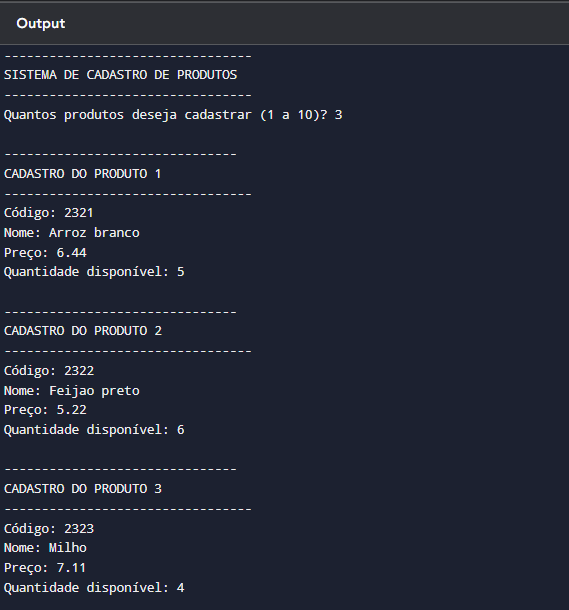
\includegraphics[width=1\textwidth]{sistemacadastro.png}
    
    % 3. A FONTE SEMPRE ABAIXO (com tamanho menor)
    \vspace{0.2cm}
    \par{\small Fonte: Autoria própria (2026).}
\end{figure}

\begin{figure}[H]
    \centering
    % 1. O TÍTULO SEMPRE ACIMA
    \caption{Interface do compilador online mostrando o resultado do processo.}
    \label{fig:compilador}
    
    % 2. A IMAGEM CENTRALIZADA
    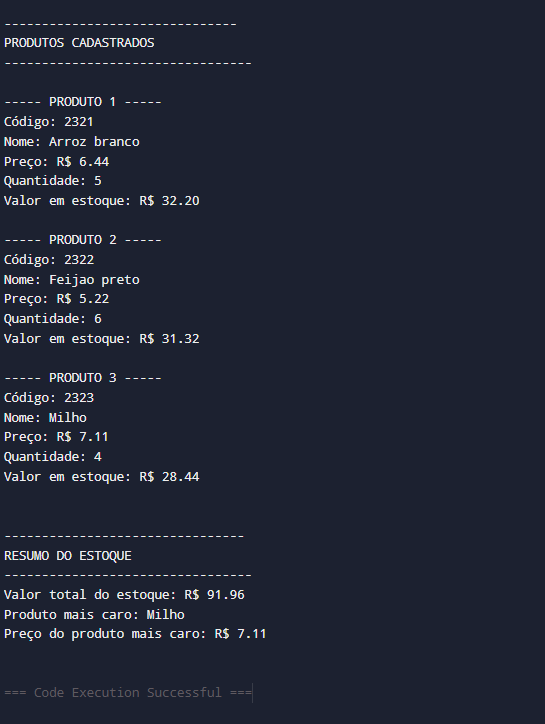
\includegraphics[width=1\textwidth]{resultadofinal.png}
    
    % 3. A FONTE SEMPRE ABAIXO (com tamanho menor)
    \vspace{0.2cm}
    \par{\small Fonte: Autoria própria (2026).}
\end{figure}


% --- 6. REFERÊNCIAS ---
\section{CONCLUSÃO}

Durante o desenvolvimento da atividade, foi criado um sistema de controle de estoque em linguagem C, permitindo o cadastro, consulta e gerenciamento de produtos. Para sua construção, foram utilizados conceitos de programação estruturada, como estruturas , vetores, funções, entrada e saída de dados, além de bibliotecas básicas da linguagem. Além de desenvolvidos melhores noções da produção de relatórios acadêmicos seguindo as normas padrão da ABNT (Associação Brasileira de Normas Técnicas).

As principais dificuldades encontradas estiveram relacionadas com a implementação das funcionalidades de forma correta. Com a realização da atividade, o grupo ampliou seus conhecimentos sobre programação em C, aprendendo a aplicar conceitos teóricos vistos durante os estudos em sala, desenvolver a lógica de programação e estruturar melhor um sistema para resolver problemas do cotidiano relacionados ao controle de estoque.

\end{document}